%\documentclass[conference,compsoc,a4paper]{IEEEtran}
\documentclass[10pt,conference]{IEEEtran}

\usepackage{array}
\usepackage[utf8]{inputenc}   % <<<<< Linux
\usepackage[nomain,acronym,xindy,toc]{glossaries} 
\usepackage{tabularx} 
\usepackage{float}

\usepackage{cite}    
\usepackage{graphicx,flafter}
\graphicspath{{../tese2/}}

\usepackage{color, colortbl}
\definecolor{Gray}{gray}{0.9}

\usepackage{url} 



\hyphenation{op-tical net-works semi-conduc-tor}
\loadglsentries[main]{xacronyms}

\newcolumntype{Y}{>{\centering\arraybackslash}X}
\newcolumntype{M}[1]{>{\centering\arraybackslash}m{\linewidth/#1}}

\begin{document}


\title{Hyper-linked Communications: WebRTC enabled asynchronous collaboration}

\author{\IEEEauthorblockN{Henrique Rocha}
\IEEEauthorblockA{INESC-ID / Instituto Superior T\'{e}cnico\\
Av. Prof. Dr. Anibal Cavaco Silva\\
2744-016 Porto Salvo, Portugal\\
Email: henrique.rocha@tecnico.ulisboa.pt}
\and
\IEEEauthorblockN{Ricardo Lopes Pereira}
\IEEEauthorblockA{INESC-ID / Instituto Superior T\'ecnico \\
Av. Prof. Dr. Cavaco Silva\\
2744-016 Porto Salvo, Portugal\\
Email: ricardo.pereira@inesc-id.pt}
}

\maketitle

\begin{abstract}
The Hyper-linked communications concept applies much of the hypermedia concepts, widely used on Web content, to the communication realm.
This paradigm allows to synchronize, structure and navigate communication content integrated into voice and video calls.
Voice and image together can express emotions like no other medium can. With hypermedia concepts, we can add more value to conference calls.

This paper describes the design, implementation and evaluation of a hyper-linked communication platform targeting the web platform and making use of \emph{WebRTC} technology.
Our prototype provides a hyper-linked, non-linear, multi-party video conferencing platform with support for multiple media types, collaborative text editor, time annotations, instant messaging and a mechanism to superimpose hyper-content to video.

Our prototype was built using a hybrid peer-to-peer and client-server architecture, resorting to open source software.
Usability tests using 20 users evaluated our prototype positively: 100\% considered it innovative and 95\% recommended its use. 
From a deployment point of view, our performance tests showed that our solution was expensive to scale up, even though the cost could be significantly lower by disabling some of the functionality.


\end{abstract}

\IEEEpeerreviewmaketitle

\section{Introduction}
\label{chapter:introduction}


As communications technologies appeared, we adapted the way we communicate. 
Multi-party video conference is today a commonly used tool in the enterprise, academia and personal live.
The \gls{WWW} has made us familiar with the concept of text hyper-media, in the form of hyper-links.
\gls{IPTV} and video hosting platforms, such as Youtube, made non-linear video watching a common practice.
The later also use the concept of hyper-links superimposed over videos.
However, these three concepts, video-conferencing (which is real-time), non-linear video watching and hyper-media, have largely remained independent concepts.




The purpose of this project is not the replacement of the current video and audio communications, but to enrich them with hyper-media content and make them a more natural and easy to learn process. 

The advent of \gls{WebRTC}, currently available on the major web browsers, made it possible to develop video conference web applications without plugins, greatly increasing the range of what can be implemented using web technologies.
		
    Furthermore, real time communication applications can make a significant difference on business, education and health sectors by providing tools for developing teaching and learning online, teamworking and socializing web applications.

\subsection{Proposed Solution}
\label{section:proposed}

	Our goal in this project is to develop an application targeted to the web platform, resorting to \gls{WebRTC}, that leverages the hyper-linked communications by providing a video conference environment enriched with interactive and non-interactive discrete media types such as images, subtitles, forms and all types of content that can be added using \gls{HTML}5, \gls{CSS}3 and \emph{JavaScript} including continuous media types such as video, music and animations.

	One of the key features of this project is the ability to navigate in time in order to reproduce the conversation again or introduce hyper-content to it such as time annotations, interactive lists of topics and subtitles. In this context we also provide a simpler method for creating and synchronizing hyper-content using \gls{QR} codes.

	In addition to this conference environment, which provides different functionalities than traditional conference environments such as \emph{Skype} and \emph{Google Hangouts}, we also enable a collaborative text editor and a chat that supports sending time hyper-links and files to conference participants.

	Furthermore, another relevant feature is the possibility to compose multiple video streams into a single one, which enables adding more users to conference rooms without impacting on clients performance. Users can change to individual streams on demand or automatically to the talking users.
        


\emph{WebRTC} technology allows real time communications between web browsers without the need to install additional software. The nature of web browser applications already follows the hypermedia concept, which makes \emph{WebRTC} the ideal technology to apply the hyper-linked communications concepts.
The web browser platform provides an abstraction layer that makes it possible to create applications that run independently from the operating system.
The native support for \emph{WebRTC} in operating systems extends its usage to outside the web browser, allowing for the exploration of functionalities for which web browsers provide poor support, such as video recording and massive information storage.

\subsection{Thesis Contribution}
\label{section:contribution}

Making it clear, this project aims to complement current audio, text and video communications in order to create rich and collaborative interfaces with the ability to add more content on a future time (\emph{e.g.} creating time annotations for improving content search) in order to increase its value. It is also important to highlight another goal of this project which is the ability to navigate in time by rewinding communications, fast-forward and jump to certain points.

	We have presented an architecture that can meet our goals, implemented the respective prototype and tested it with real users and performance benchmarks.

	According to Martin Geddes, the quality of the interaction worsens as the number of users increase\cite{geddes}. In our testing phases we will quantify and qualify the impact of increasing users on the interface and performance of our prototype. 

	All the problems faced during the development and limitations were reported on the thesis so that a future project better then ours can be easily and better developed.

The remainder of this paper is organized as follows.
Section \ref{chapter:relatedwork} provides an overview of previous work in the field.
Section \ref{chapter:architecture} describes the requirements we defined for our system and architecture for fulfilling them.
The choices performed for the implementation of our prototype are presented in Section \ref{chapter:implementation}.
In Section \ref{chapter:evaluation} we present the evaluation tests performed and their results.
Section \ref{chapter:conclusion} summarizes the work developed and proposes future work.









\section{Related Work}
\label{chapter:relatedwork}


Since the early days of video technology, one of the problems raised consisted on how to add more information onto video without generating multiple versions. This section examines technologies that allows different ways to present multimedia content in such a way that it change based on synchronization amongst other multimedia elements or user interaction.

\emph{Hypertext} is a type of text that provides links to texts or other types of content, these links are known by \emph{hyperlinks}. \emph{Hypermedia} is an evolution of \emph{hypertext}, it includes audio, images, text and video. 

\emph{Hypermedia} concept brings the possibility to organize and overlay multimedia elements into a nonlinear linear structure.

In the beginning of analog video technology, the navigation over it was quite limited to simple operations such as play, stop, rewind and fast-forward. As video started to be digitalized, new operations over video emerged, such as random jumps and chapter navigation through interactive menus present on \gls{DVD}.

%RP depois disto falta uma introdução a explicar que precisas de controlar a apresentação e execução de diversos conteúdos e que para isso vais precisar de uma tecnologia que permite sincronizar e controlar. Esta secção examina isso.

Some \gls{MPEG} implementations, like \cite{embedded}, added hypermedia information to empty space present on \gls{MPEG} frames in order to provide interactive television, modifying the \gls{MPEG} encoder and decoder in order to handle hypermedia content.
%RP esta última frase, com detalhes de implementação fica algo deslocada antes de apresentares os exemplos de hypermedia. Talvez deslocar para mais tarde.
Hypermedia is a concept that holds the promise of future technology and features but it is also already present in our daily lives.
%RP por exemplo na publicidade no youtube

  Subtitles are an example of information that might be required.
  The need to translate movies, raised the problem whether it is appropriate to change the original video or audio. For example, subtitles should be an entity independent from the video, in order to be personalized or replaced easily.

  \gls{SAMI}, and \gls{SRT} are two of the multiple formats for subtitles commonly supported by video players. Although those formats have styling available, they are quite limited to text. 

  Hyper-video is a kind of video that contains links to any kind of hypermedia, including links to skip part of it. An example of hypermedia application could be a search engine over hypermedia content, like subtitles, in order to jump to a specific time in a video or audio track. \emph{HyperCafe}~\cite{hypercafe} was an experimental project to expose hyper-video concepts that consisted of an interactive film that enabled switching between different conversations taking place inside a cafe.
 
  Detail-on-demand is a subset of hyper-video that allow us to obtain additional information about something that appears along the video, like obtaining information about a painting that appears in a particular segment. \emph{Hyper-Hitchcock}~\cite{hitchcock} is an editor and player of detail-on-demand video.

  In order to navigate through a dynamic video, we must be aware of time synchronization and the multiple time flows, it ils important that all time, causality and behavior rules are well defined.
  %RP one must be aware? O utilizador? Ou queres dizer que é preciso definir as relações? O que falas a seguir é sobre linguagens para isso.
  
  \emph{HyVAL}~\cite{hyval} is an \gls{XML} based language that was proposed for modeling composition, synchronization and interaction of hypermedia. HyVAL defines defines video structure, internal video and external media objects. 
  \emph{HyVAL} uses a primary video stream, around which all other elements are organized and synchronized.
  \emph{HyVAL}'s video structure object defines a structure derived from traditional video, which divides video into segments, scenes, shots and frames hierarchically. 
  This approach is quite restrictive if we want to apply hyper-video concepts to videos that do not follow this structure. External media objects are linked by primary video, those objects can represent other videos, images, text, animation and sound.
  %RP não percebo bem a última frase. O que é primary video?

  \gls{SMIL}~\cite{smil} was introduced to describe temporal behavior of multimedia content, in particular, it could be used to overlay subtitles on films. With \gls{SMIL} it is possible to synchronize multiple videos, either in parallel or in sequence, reproduce a different audio track, overlay user interface elements with hyper-links, among multiple other features.
  %RP synchronize multiple sections of video? vários videos apresentados em simultâneo?

  \gls{SMIL} is an \gls{XML} based language that defines twelve modules: \emph{Animation}, \emph{Content Control}, \emph{Layout}, \emph{Linking}, \emph{Media Objects}, \emph{SmilText}, \emph{Meta Information}, \emph{Structure}, \emph{Timing}, \emph{Time Manipulations}, \emph{State} and \emph{Transitions}.


\begin{itemize}

  \item The \textbf{Animation} module contains elements and attributes that define a time based mechanism for composing the effects of animations. For example, this module can perform changes on \gls{XML} or \gls{CSS} attributes like color and dimensions.  

  \item The \textbf{Content Control} module contains elements and attributes that provide optimized alternatives for content delivery. For example, it could be used to change audio language in function of user's nationality, for videos with multiple audio channels.

  \item The \textbf{Layout} module contains elements and attributes for coloring and positioning media content. Other layout mechanisms are also possible, such as \gls{CSS}.

  \item The \textbf{Linking} module contains elements and attributes for navigational \emph{hyperlinking}. Navigation can be triggered by events or user interaction.

  \item The \textbf{Media Object} module contains elements and attributes for referencing rendering behavior of external multimedia or control objects.

  \item The \textbf{SmilText} module contains elements and attributes that define and control timed text. For example, this module could be used to create labels and captions.

  \item The \textbf{Meta Information} module contains elements and attributes that allows describing the \gls{SMIL} document. For example, this module could be used to define movie details such as category, director, writers and cast.

  \item The \textbf{Structure} module defines the basic elements and attributes for structuring \gls{SMIL} content. This module defines a \emph{head} element that contains non temporal behavior information defined by  \emph{Meta Information}, \emph{Layout} and \emph{Content Control} modules. This module also defines the \emph{body} element, where all temporal related module information is contained.

  \item The \textbf{Timing} module is the most important module on \gls{SMIL} specification. Due to its complexity, it is divided into seventeen sub-modules for coordination and synchronization of media over time. The three main elements are \emph{seq}, \emph{excl} and \emph{par}, that, respectively, play child elements in sequence, one at a time and all at the same time. 

  \item The \textbf{Time Manipulations} module adds time behavior attributes to \gls{SMIL} elements, such as speed, rate or time.

  \item The \textbf{State} module defines attributes that define the state of \gls{SMIL} elements, such as element visibility, current element time, amount of repeated loops, playing state and many others.

  \item The \textbf{Transitions} module defines attributes and elements for transitions across multiple \gls{SMIL} elements according to the \emph{Timing} module.

\end{itemize}

The \gls{DOM} is a standard \gls{API} that allows easy management of documents that are organized in a tree structure, by providing \gls{CRUD} operations over its elements and their attributes. \gls{DOM} makes it easy to inter-operate between imperative and declarative programming languages~\cite{dom}.
%RP não arranjas uma referência para o dom?

Like \gls{DOM}, \gls{SMIL} \gls{DOM} is an \gls{API} for \gls{SMIL} documents. Allowing \gls{CRUD} operations over \gls{SMIL} documents is an important feature for extending \gls{SMIL} capabilities, for example for creating non-linear animations and triggering external events like \emph{JavaScript} functions.  


  \gls{SMIL}'s modules can be used to synchronize and animate \gls{XHTML} and \gls{SVG} elements.
  %RP ``are used'' ou ``can be used''?
  
  \gls{SMIL} fits our goals for creating a multimedia rich hyper-call, but it lacks on browser compatibility. Ambulant \cite{ambulant} was one of the SMIL players that were developed for browsers, although this player implements most of \gls{SMIL} 3.0 \cite{smil3} specifications, it needs to be installed on browsers as a plug-in.

  SmillingWeb \cite{smillingweb} attempts to implement a cross platform multimedia player designed for \gls{SMIL} 3.0 presentations with \emph{JavaScript} and \emph{jQuery} which, unlike \cite{ambulant}, does not require a plug-in to be installed and should not have incompatibility issues. 
  SmillingWeb already takes advantage of \gls{HTML}5 and \gls{CSS}3.
  It takes into account unsupported web browsers through the use of \emph{Modernizr}\footnote{\url{http://modernizr.com/}(accessed June 2, 2015).}, a simple \emph{JavaScript} library that may require plug-ins if new features are not supported.  
  But SmillingWeb just implements a subset of \gls{SMIL} 3.0 and their scheduler engine loads the \gls{SMIL} file only once, which could raise problems when dealing with \gls{SMIL} changes due to real time communications.
  Another problem with SmillingWeb is pre-loading and playing elements at the correct interval of time, which is not always possible due to high latency networks leading to  pauses during playback.

% XXX
  %RP fazes uma mudanças de tema muito bruscas. Podes usar \subsubsection ou \paragraph para dividir isto melhor. E uma frase entre temas a servir de ``cola'' ou ``separação'' também não fica mal


  An alternative to \gls{SMIL}'s \emph{Layout} module is to use \gls{HTML} which is a markup language based on \gls{XML} that is used for creating web pages. \gls{HTML} alone is a very poor language when we are focused on visual appealing and interactive web pages. Languages like \gls{CSS} and \emph{JavaScript} are typically used along with \gls{HTML} for improving the interaction and appearance of a web page. 


  %RP esta parte está um pouco confusa. Primeiro falas de smil, depois de html, depois de smil novamente. Devias agrupar tudo. Devias agrupar as soluçoes por tecnologia. Se preciso, primeiro fala de html, css, etc, e depois de smil e das implementação de smil (incluindo as que são implementadas em html e js).
  
  \gls{CSS}'s goal is to separate the structure of an \gls{XML} document from its appearance. \gls{CSS} defines styles for \gls{XML} tags based on their name, class, identifier or position.
  Besides static styling \gls{CSS} also supports animation and transitions leading to more dynamic content.
  %RP Tens muitas alturas em que não começas frases novas. Usas virgulas para separar conteúdo que não faz sentido ficar na mesma frase pois começa com um novo sujeito seguido de verbo.

  \emph{JavaScript} is an imperative object-oriented language based on \emph{ECMAScript}. It is used mainly on client-side and executed by a web browser. \emph{JavaScript} has its own implementation of \gls{DOM} and one of its advantages is the ability to download and execute code on-the-fly without the need of pre-installed plug-ins.

  \emph{JavaScript} has compatibility issues among the different web browsers, leading to different behaviors. To solve that problem, there are libraries written in \emph{JavasSript}, namely \emph{jQuery}, that implements the same functionality for multiple browsers, masking most of the incompatibility issues.

  With the emergence of \gls{HTML}5, tags like \emph{video}, \emph{audio} and \emph{track} allow us to play video with multiple \emph{codecs}, audio and subtitles in \gls{WebVTT} format. Another important tag is \emph{canvas} that allows drawing graphics with \emph{JavaScript} on a rectangle within a web page.

  For example, with \gls{API}s like WebGL\footnote{\url{http://khronos.org/webgl/}(accessed June 2, 2015).}, it is now possible to manipulate a three dimensional environment in the context of a hyper-call. Another example would be a collaborative spreadsheet using \gls{WebRTC}. With this, hyper-calls are not limited to only audio, image, text and video, but also interaction with complex graphical user interfaces that changes over time.


  \gls{SVG} is an \gls{XML} based format that incorporates the animation module of \gls{SMIL}. Currently, \gls{SVG} allows adding movement and animating attributes of elements. When embedded on \gls{HTML}5, it allows dynamic changes to inner content in real time through the \gls{DOM} \gls{API}. Besides that, it also allows calling \emph{JavaScript} functions on events such as animation end, mouse over and mouse click.
  
  Back in 1995, \emph{flash}\footnote{\url{http://www.adobe.com/products/flash.html}(accessed June 2, 2015).} was developed for web-based animations. Introducing video support in 2002, \emph{flash} started to grow after that. Competitor's players, at that time were focused on playing video and audio, while \emph{flash} had vector graphics and focused on streaming \emph{on-demand} video across multiple platforms. \emph{VP6} was their choice of video \emph{codec}, providing half the video size (in Byte) for the same quality and providing video quality adjusted to \emph{Internet} connection latency. 
  In 2010, \emph{Adobe Flash} was the most widely used applications for reproducing live broadcast and recorded video \cite{flashvideo}, it supports progressive video download using \gls{HTTP} and streaming using \gls{RTMP}.

  \gls{RTMP} is a \gls{TCP} based protocol used for streaming audio, video and data between a \gls{FMS} and \emph{flash} players. A bidirectional connection is established between the two in order to allow real time communications. A \emph{flash} player can stream a webcam video to a \gls{FMS} using \gls{RTMP} or it can request a video stream to \gls{FMS} that can either be a pre-recorded stream, live stream or data. Multiple \gls{FMS} servers can be used in parallel to increase capacity and handle more streams simultaneously.
  %RP chained ou usados em paralelo?

  \gls{FMS} can stream video and audio to one or more subscribers by sending a separate copy for each subscriber. With \gls{RTMFP} it is possible to stream video directly between \emph{flash} players, allowing a publisher to break up a stream into pieces that can be cooperatively distributed in a P2P mesh. \gls{RTMFP} uses \gls{UDP} to speed packet delivery, which although it is not reliable, is well suited for video streaming. Like \gls{WebRTC}, \emph{flash} players also need to apply techniques like \gls{STUN} and \gls{TURN} for \gls{NAT} traversal.

  Although \gls{HTML}5, \emph{JavaScript}, \gls{CSS} and \gls{WebRTC} implement some of \emph{flash}'s features, it does not mean that \emph{flash} will be replaced soon.
  Instead, both technologies can be used to develop rich \emph{Internet} applications.
  It is also important to note that \gls{HTML}5 is better supported in mobile devices than \emph{Adobe Flash}. 

  Like \emph{Flash}, \emph{Microsoft Silverlight}\footnote{\url{http://www.microsoft.com/silverlight/}(accessed June 2, 2015).} is a cross browser plug-in and platform that is used to develop rich \emph{Internet} applications. It supports vector graphics, animation and video. Compared to \emph{flash}, which uses \emph{ActionScript}, \emph{Silverlight} applications can use languages like C\#, \emph{VisualBasic} and \gls{XAML}. \emph{Silverlight} uses a technique called \emph{Smooth Streaming} from \emph{IIS Media Service} that consists on delivering video in real time with adjusted quality in function of bandwidth variations and \gls{CPU} usage.

  Using technologies that relies only on web standards, like \gls{CSS}, \gls{HTML}5, \emph{JavaScript} and \gls{SVG}, will make possible to develop an application that solves our problem with the advantage of being compatible with a greater amount of web browsers.








\gls{WebRTC} is an open source technology that defines a collection of standard protocols and \emph{JavaScript} \gls{API}s for web browser based real time communications without installing any additional application or plug-in. 

\gls{WebRTC} uses \gls{SDP} \cite{rfc4566} to define peer connection properties such as types of supported media, \emph{codecs}, protocols used and network information. An \gls{SDP} offer describes to other peers the expected type of communication and its details, such as used transport protocols, codecs, security and other.


Some operating systems such as \emph{Android}, \emph{iOS}, \emph{Linux}, \emph{OSX} and \emph{Windows} implement native \gls{WebRTC} libraries, extending the usage of \gls{WebRTC} to applications outside the web browser. This native support can help to implement applications that record video and audio streams for further playback.

However, \gls{WebRTC} by itself does not define how users get to know each other nor how information flows between users. For this reason, we have studied the multiple ways we could implement this \emph{get-to-know} mechanism which is known as signaling protocol.


  Signaling is the process by which applications exchange connection information about peers and servers, their capabilities and meta-data.
  In particular, \gls{WebRTC} does not implement signaling, as different applications may require different protocols and there is no single answer that fits all problems.
  As a consequence, multiple options are available for filling the missing \gls{WebRTC}'s signaling component, which can be performed using \gls{SIP}\cite{rfc3261}, \gls{XMPP}, \emph{WebSockets}, \emph{Socket.io}\footnote{\url{http://socket.io/}(accessed June 1, 2015).}, \gls{SigOfly}\cite{sigofly} or by implementing a custom protocol.

 
	\emph{Hypermedia} concept brings the possibility to organize and overlay multimedia elements into a nonlinear linear structure holding the promise of future technology and features. Languages such as \gls{SMIL}~\cite{hyval}, \emph{HyVAL}~\cite{hyval} and \gls{HTML} can be used to implement the \emph{Hypermedia} concept. Two examples of applications that captured our attention were \emph{HyperCafe}~\cite{hypercafe} and \emph{Hyper-Hitchcock}~\cite{hitchcock} which explored interactive video features.

 
\subsection{Extending collaboration tools with time manipulation}
\label{collab}

Real time collaboration applications have become a huge help on team tasks, providing a great boost on business, research and investigation velocity.

 Our first concern on real time collaboration applications is the data storage and representation. Storing multimedia content on a web client is not a viable solution because the local storage is limited to at most five megabytes per origin. Additional servers will be required to process and record the large amount of data generated by audio and video streaming.
 
\gls{KMS} supports streaming over \emph{WebRTC}. Another important component of \gls{KMS} is \emph{Kurento Repository}, which supports recording and playing directly from \emph{MongoDB}. That is important for providing a scalable media storage. 
	
     \gls{OT} technology was originally developed for consistency maintenance and concurrency control over distributed objects.
     \gls{OT} algorithms are mainly used in collaborative applications such as distributed document edition.

	Among mutiple \gls{OT} platforms and libraries we present \emph{ShareJS}\footnote{\url{http://sharejs.org/}(accessed June 2, 2015).}, \emph{TogetherJS}\footnote{\url{http://togetherjs.com/}(accessed June 2, 2015).}, \emph{Goodow}\footnote{\url{http://realtimeplayground.goodow.com/}(accessed June 2, 2015).}, \emph{Etherpad Lite}\footnote{\url{https://github.com/ether/etherpad-lite}(Accessed 20 March 2016)} and \emph{otJS}\footnote{\url{http://operational-transformation.github.io}(accessed March 10, 2016)}.


	\emph{otJS} is a \emph{JavaScript} library that only implements operation transformations over plain text on the client side and requires implementing the content's persistent storage. Besides this drawback, this library is very flexible because it is not tied to a specific database or server side technology.
        

\subsection{Streaming and Recording}\label{recstream}~\\
	If, for instance, one wants to rewind a real time video, recordings will be needed from whom is streaming the video. 
 Our first concern on real time collaboration applications, besides the communication itself, is the data storage and representation. Storing multimedia content is not a viable solution because most browsers recommend limiting local storage to at most five megabytes per origin\footnote{\url{http://www.html5rocks.com/en/tutorials/offline/quota-research/} (accessed May 13, 2016)} .

 	In order to provide a way to record and playback streams, additional servers will be required to process and record the large amount of data generated by audio and video streaming.

 \gls{RTP}\cite{rfc3550} is used for streaming audio and video over \gls{IP}.
 Multimedia content is transported on the payload of \gls{RTP} messages, that contain headers for payload identification. \gls{RTP} is independent from its payload type, allowing it to transport any kind of encoded multimedia. A sequence number is used for sorting received packets.

\gls{RTCP} is used for controlling \gls{RTP} multimedia streams, it provides bandwidth statistics and control information that can be used for changing the quality of the stream in real time.

  \gls{RTP} allows to change its requirements and add extensions to it with profiles. One of the most used ones is the \gls{RTP} profile for audio and video \cite{rfc3551}, which lists the payload encoding and compression algorithms. This profile also assigns a name to each encoding which may be used with other protocols like \gls{SDP}.
  Another profile for \gls{RTP} is defined by \gls{SRTP}, which provides encryption, authentication and replay protection for \gls {RTP} traffic. The analogous secure protocol for \gls{RTCP} is \gls{SRTCP}.

  Both \gls{SRTP} and \gls{SRTCP} use \gls{AES} by default, which is a symmetric-key algorithm for data encryption. Each packet is encrypted using a distinct key-stream, as otherwise, using a single key-stream with \gls{AES} on \gls{CBC} would make it impossible to recover from packet loss.

  Two key-stream generators for \gls{AES} were defined: \emph{Segmented Integer Counter Mode} and \emph{f8-mode}. If a packet is lost, there is no impact on other packets, as the initialization vector is obtained through those key-stream generators and it is fixed for each packet.
  %RP isto está tudo no RFC3550? Se não, faltam muitas citações.
  %HR esse RFC é grande


  \gls{RTP} recorders are independent of payload encoding, they do not decode \gls{RTP} packets, they record packets instead, allowing to record all video and audio formats even if they're encrypted.

        %RP lá vais tu mudar de tema da conversa sem explicar porquê....
        Even though one on one calls are common, there are occasions when several people take part of the same video call.
	Multi-party video calls can be achieved on \gls{WebRTC} by streaming video from each participant to all the other participants. Although this works, the bigger a conference room is, the bigger is the used bandwidth to stream video to all participants within the conference room.
        In this scenario, a more efficient alternative to peer-to-peer is the use of a \gls{MCU}.

	\emph{Jitsi Video Bridge} \footnote{\url{http://jitsi.org/Projects/JitsiVideobridge}(accessed June 2, 2015).} receives one stream from every participant on a conference, either from a \emph{jitsi} client or a \emph{WebRTC} application, and redirects it to all the other conference participants, reducing the amount of data that each peer sends. Although all the participants still need to download all the streams from the \emph{Jitsi Video Bridge} server, typically download rates are much bigger than upload rates, making this solution more feasible.
	\emph{Jitsi Video Bridge} uses \gls{XMPP} as a signaling protocol and its \emph{colibri} extension \cite{xep0340} to reserve channels for video transmission. Despite this choice for signaling protocol, \emph{Jitsi Video Bridge} also supports \gls{SIP}.

	
	  \gls{KMS} supports trans-coding, group communications, recording, mixing, broadcasting, applying filters and performing image and sound analysis (for example it allows face and QRcode detection). \gls{KMS} functionalities are exposed through \emph{JSON-RPC} over \emph{WebSocket}.
          There are three clients available: \emph{JavaScript} client for web browsers, \emph{Java} client for \emph{Java EE} servers and \emph{JavaScript} client for \emph{Node.js} servers. 
	\gls{KMS} supports streaming over \emph{WebRTC}, \gls{HTTP} and \gls{RTP} endpoints. Another important component of \gls{KMS} is \emph{Kurento Repository}, which supports recording and playing directly from \emph{MongoDB}. That is important for providing a scalable media storage. Unlike \emph{Jitsi Video Bridge}, \gls{KMS} does not enforce a specific signaling protocol.
	











\section{Architecture}
\label{chapter:architecture}

Taking into account the goals of this project and all the technology presented so far. Our proposal is the development of a web application that provides communication and collaboration features in real time.

\subsection{Requirements}
\label{chapter:requirements}
In a general way our system's goal is to provide a multi-party video and audio conference environment that supports chat, time manipulation, collaborative text edition and hyper-content creation.

%RP isto pode ser muito expandido. Podes começar por descrever os goals (mais alto nível): audio e video conferência multi-party, possibilidade de rever o que foi dito antes, chat, etc etc.
% Só depois traduzes isso em requisitos, tanto funcionais como não funcionais
% Depois apresentas a arquitectura, fazendo um paralelo entre os módulo e escolhas realizadas e quais os requisitos que cada um deles satisfaz. 

For our system, our application must provide: a simple way to send instant text messages to the conference participants, ability to recording and playback recorded video including all the hyper-content displayed at that time, mixing multiple user streams into a single stream, create annotations associated to a specified time, allow users to superimpose hyper-content to video given a range of time, search every objects related to a conference room such as hyper-content, time annotations and users, share files and time links among users, sound detection for showing the current speaker, provide a collaborative text edition tool, interpret \gls{QR} codes in order to ease content creation and support database replication.
%RP capacidade de lidar com NAT

	Moreover we allow clients to discover chat rooms and other clients by navigating on the web pages provided by our web server. In addition users can create rooms for multi-party audio and video communication communication which is achieved by using \gls{WebRTC}'s \emph{PeerConnection}.
        %RP falas em peerconnection, mas na figura 3.1 apenas há um cliente, o que obviamente impede mostrar a comunicação entre peers.
        %RP acho que podes fazer outro diagrama com a comunicação entre os vários componentes, onde apareceriam vários clientes. A aí indicas o tipo de ligação entre cada par de componentes (HTTP, PeerConnectino, websocket, MediaStream ...)
        
\subsection{Modules}
In this section we present the several modules that were designed in order com fulfill the set requirements.
	Figure~\ref{fig:modules} presents the structure of our system which was divided into six modules:


\begin{figure}
	\centering
	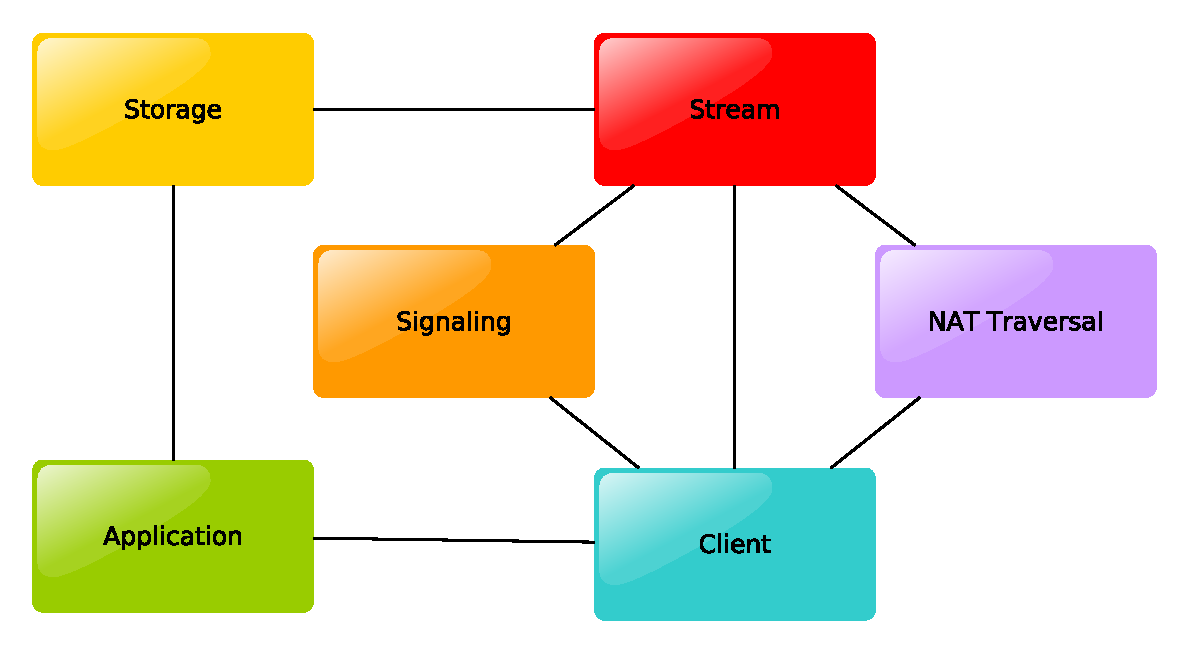
\includegraphics[width=\linewidth]{figures/modules.pdf}
	\caption{System Modules}
    \label{fig:modules}
\end{figure}



\begin{itemize}

\item \textbf{Application module} - responsible for providing information about the relevant modules (\emph{NAT Traversal} and \emph{Signaling}) and user interface to the \emph{Client} in the form of web pages in \gls{HTML} and \emph{JavaScript} libraries through \gls{HTTP}.
 
\item \textbf{Signaling module} - responsible for \emph{Client} and \emph{Stream} coordination which will be performed using \emph{WebSockets}.

 \item \textbf{NAT Traversal module} - \gls{STUN} and \gls{TURN} techniques used by \emph{Client} and \emph{Stream} modules during the \emph{Signaling} phase which ends by establishing the connection between them.

 \item \textbf{Stream module} - responsible to deliver and receive multimedia content from the \emph{Client} using \gls{WebRTC}. 

 \item \textbf{Storage module} - provides two main functionalities: store the model information and media recorded. This is the single module responsible for persistent storage. It stores user and communication data as well as all the data required among user sessions. It is also use to store all the communication streams, so that they can be viewed later.

 \item \textbf{Client module} - responsible for the interaction with the user.

\end{itemize}

%RP Acho que podes escrever muito mais sobre cada componente. Isto está muito curto. Fala de algumas das funções que proporcionam. Vê o que fiz com o Storage Module

%RP também podes fazer um diagrama com vários utilizadores e mostrar quais os streams que vão de e para cada um (mostrar a mistura de som, video, etc).

 
\subsection{Implementation Proposal}
The infrastructure is composed by: web server, stream server, signaling server, database and video repository.
%RP tens da fazer o paralelo entre isto e os componentes apresentados na secção anterior. O mesmo com a imagem, que parece não estar relacionada. Podes colocar os elementos na mesma posição, ou dentro das caixas da imagem 3.1

\begin{figure}[H]
	\centering
	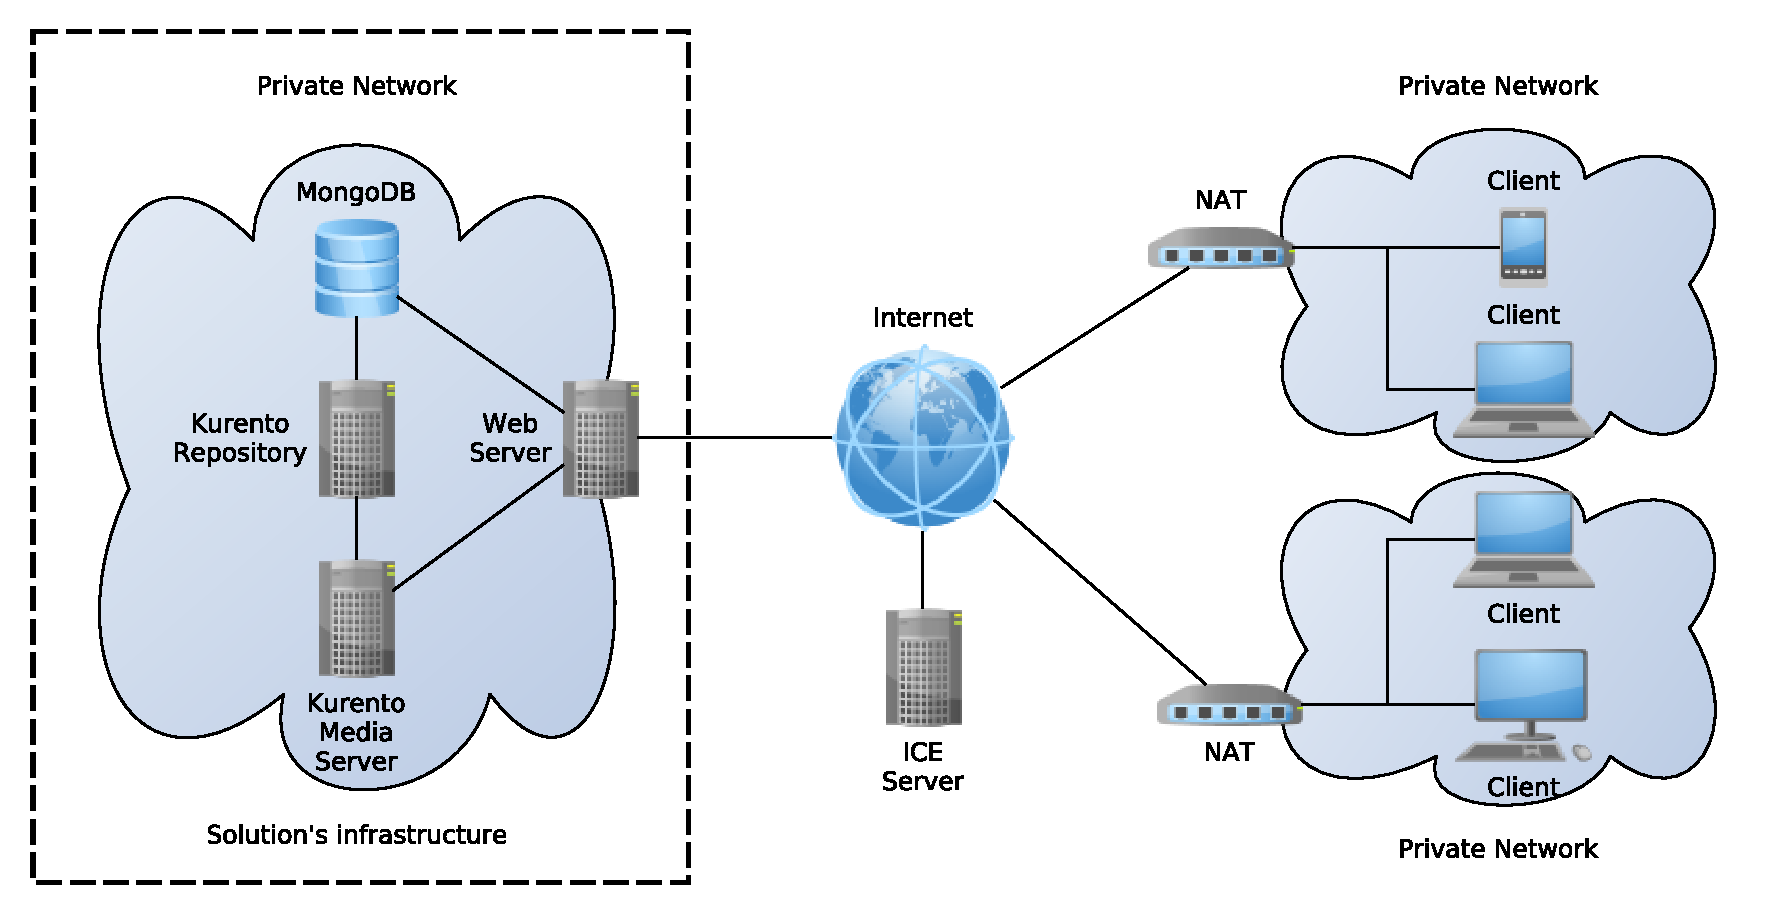
\includegraphics[width=\linewidth]{figures/infrastructure.pdf}
	\caption{System Infrastructure}
\end{figure}

In order to simplify our solution, we propose that the \emph{Application}, \emph{Signaling}, \emph{Stream} and \emph{Storage} modules be implemented within the same server application, so it could be easy to deploy as a single image. To this set of modules, we often call \emph{backend}.

	\subsubsection{Security and authorization}

Having established that the \emph{backend} modules are placed in the same machine, that helps controlling which resources the client has permission to access as those modules are seen as a private network.
%RP na mesma ``server application'' ou ``machine''? São coisa diferentes! Apresentas vantages de instalar tudo na mesma máquina mas não falas das desvantagens. Menor escalabilidade parece-me ser logo uma delas. Na figura 3.2 aparecem várias máquinas!

To qualify the above we provide public access to \gls{HTTP} server ports, maintaining the access to other components restricted through firewall rules.
%RP qualify?
%RP Imagem com firewall e estes portos? Mas isto já me parece muito detalhe de implementação.
In relation to the database there is no directly access from the outside. All the database information is accessed via our application server which validates the permissions of users on our system.

On the other hand, the access to our streaming servers is also restricted, but clients can connect to them after concluding the signaling phase. This signaling phase may or not proceed in function of the client access permissions. For example, if a user is trying to access a private conference room that he is not a member of nor has an invitation link for, the signaling server refuses to start the signaling phase and the user cannot access the streaming server.

The placement of our streaming servers inside a \gls{NAT} also has an important role with respect to external misuse prevention. Otherwise, placing our streaming servers could allow external clients to perform their own signaling protocol and, as a consequence, use our infrastructure without our consent.

\subsubsection{Client connections}
	Although the delegation of processing work to clients can improve our system's scalability, we are concerned about using the least resources possible on the client side, as huge resource consumption may drain battery very fast or may even be impossible to run on mobile devices. We are aware that streaming video from clients is already a very intensive task which we cannot avoid but can improve by delegating the most intensive tasks to our servers. 


	In this context, with a centralized approach, each client must only have one \emph{PeerConnection} to our streaming server and content shown to them is changed on demand either being it an individual or a composite view. Otherwise clients could follow a peer-to-peer connection which would result on maintaining more connections and performing the composition of videos on client side.

	The composition of streams on client side is performed by receiving streams with the best quality possible but, due to undersizing the video of clients into a smaller region, this would result on wasting bandwidth on a quality that is not needed.

	Although the peer-to-peer approach could be used on our system, we conclude that we need to record the video on our streaming server because web clients have a very limited storage and peer disconnections may result on recorded video loss. 

	The same can be concluded to instant message delivery, each client must have only one \emph{WebSocket} connection to the application server which consequently relays the messages to other users.

	Relaying instant messages from clients through the our web servers is easier if all clients are connected to the same server because all messages can be directly delivered without sending messages across multiple web servers. 

	In the context of this thesis, we will not implement sending messages across web servers but, in order to allow our system to scale, we will consider that all conference participants are connected to the same server and our system is scaled by having conference rooms distributed across different servers.

\subsubsection{Software choices}

Furthermore, we have taken into account the compatibility between the streaming server, database and the operation transformation solutions, in order choose the appropriate framework to implement our web server.
%RP esta secção devia começar aqui, a explicar a escolha das tecnologias/produtos a usar em cada componente. O que tens antes são pormenores que só faz sentido discutir no final. Tens de ir sempre do mais geral para o mais detalhado.

We have decided that our solution must use \gls{KMS}. Our web server could be implemented easily with \emph{NodeJS} or \emph{Java} due to the fact \gls{KMS} provides clients for both technologies. But others could also be used as \gls{KMS} also exposes their \gls{API} via \emph{WebSockets}.

Due to the fact we are going to use \gls{KMS} as streaming server solution, we could choose \emph{NodeJS} or any \emph{Java} based web framework for implementing our web application server. We have decided to implement our web server with the \emph{PlayFramework}\footnote{\url{https://www.playframework.com/}(acessed March 25, 2016)} using \emph{Java} because of our previous experience with it.

By default, \emph{Kurento Repository} is implemented over \emph{MongoDB}, for convenience our storage model will also use the same database.

Importantly, for the collaborative text editor, we have chosen \emph{OT.js} due to its server and storage implementation choice independence.

For the \emph{NAT Traversal} module a public \gls{STUN} server can be used for testing our solution. Nevertheless, we recognize that for a production environment we would need to maintain our own \gls{TURN} servers in order to ensure connectivity to all clients.

Not less important, on the client computers, both \emph{Mozilla Firefox} and \emph{Google Chrome} could be installed as web browsers. As such, both should be supported. Libraries such as \emph{jQuery}, \emph{Bootstrap}, \emph{Adapter.js}, \emph{OT.js} can be downloaded from the web server and executed on the client side using any of these two browsers.
%RP relembrar que o IE e o Safari não suportam webrtc?

\begin{table}[H]
\centering
	\caption{Application Architecture}
	\label{table:apparch}

\resizebox{\columnwidth}{!}{%
    \begin{tabular}{cccccccc@{}m{0pt}@{}}
	\hline 
	\multicolumn{8}{|c|}{\cellcolor{Gray}Application}  &\\[12pt]\cline{1-5}\cline{7-7}
	\multicolumn{1}{|c|}{jQuery} & \multicolumn{1}{c|}{HTML5} & \multicolumn{1}{c|}{CSS3 (Bootstrap)} & \multicolumn{1}{c|}{Signaling} & \multicolumn{1}{c|}{ot.js} & \multicolumn{1}{c|}{\cellcolor{Gray}} & \multicolumn{1}{c|}{adapter.js} & \multicolumn{1}{c|}{\cellcolor{Gray}} &\\[12pt]\hline
	\multicolumn{1}{|c|}{HTTP} & \multicolumn{2}{c|}{User Interface}  & \multicolumn{3}{c|}{WebSocket}    & \multicolumn{2}{c|}{WebRTC}      &\\[12pt]\hline
	\end{tabular}
}
\end{table}

%RP acho interessante o que queres fazer aqui mas acho que está mal conseguido. A linha de baixo, devia ter coisas ao mesmo nível, o que não aconteçe.
% Qual a razão para HTTP estar por baixo do jquery e user interface estar ao lado?
% Sugiro colocar a applicação no meio e as várias interfaces (webrtc, websocket e http) uma de cada lado (esquerda, baixo e direita), indicando o que fica do outro lado (outro cliente, servidor web, servidor stream, etc)

Table~\ref{table:apparch} presents the application architecture and the underlying technologies seen from the user's perspective. \emph{Adapter.js} and \emph{jQuery} will ensure that our application is compatible with the most popular web browsers.
\emph{Bootstrap} will be used to make the user interface more appellative and responsive. With \emph{Bootstrap} it is quite easy to develop applications that adapt to mobile devices with different screen sizes.
%RP bootstrap não aparece na figura!

With respect to displaying content, the synchronization between multimedia elements will be performed through chains of \emph{JavasSript} events or by specifying the interval of time which time content must be visible. Other animations can be implemented with \gls{SVG} embedded on \gls{HTML}.
%RP Caiu do céu! Tens de explicar e ligar melhor a sequencia de texto

\section{Implementation}
\label{chapter:implementation}
\subsection{Data Model}

The data model is a critical component of our solution, as a badly designed model can imply serious difficulties when implementing new features that are not part of the plans. During the course of this project, we had to redesign the model more than once in order to support new features.

In order to offer all the functionalities that we promise, some information about objects must be persistent such as users, groups,relations among users, group memberships, messages, hyper-content, recordings and collaborative editor state. For designing our model we have taken into account generic programming techniques. We observed that operations like searching for an object were quite repeated across different types of objects. 

\subsection{Signaling Protocol}


Although we have mentioned that the signaling protocol is used to establish connections between peers, on our system our media server (\gls{KMS}) is a peer that receives video streams and sends to its connected clients. 

After the web application server validates the user access, the signaling protocol allows the users to directly connect to the \gls{KMS}, which is placed in a private network, and lets the application server and users negotiate media types and encoding information to use during the conversation.

Our signaling protocol consists of sending and receiving \gls{JSON} formated messages over \emph{WebSockets} by both the application server and the client. 


When a user enters a group conference, after the page is completely loaded, a WebSocket is created to maintain a connection with our web servers. 
But before creating the web socket, we must identify the user and check if he has permissions to participate in the conference. The user identification is done by retrieving the session id from the cookie provided by the user-agent (web browser) through the \gls{HTTP} headers.
%RP não é bem o user que fornece o cookie. é o user-agent (browser). Convém ser preciso.
%HR done
The Web application server retrieves all the information needed from the database in order to check if the user has permissions to join that conference room. It is important to save the user identification before the \emph{WebSocket} connection is created because, after the handshake is performed by the \emph{WebSocket} protocol\cite{rfc6455}, the \gls{HTTP} context is lost.
%RP socket -> websocket?

At this stage, the web application's user is asked if he wants to share its camera and microphone, share screen or just receive streams from the server. 

If the user decides to share his camera or screen the user agent creates an offer, sets a \emph{local session description} to its \emph{PeerConnection} and sends it through the WebSocket to the Application Server.

The server receives and processes the offer and sets the \emph{remote session description} to its client associated \gls{WebRTC} endpoint. Then a \emph{local session description} is created on the server and sent back to the client. After that, the server tries to gather \gls{ICE} candidates.

The client receives the server answer, sets the \emph{remote session description} and gets the ice candidates from the \gls{ICE} server.
%RP tens ``ice'', ``\gls{ICE}''. Acho que também já vi ``ICE''. Convém ser sempre igual!

Subsequently, after a while both the server and client receive the \gls{ICE} candidates that allow the client to connect directly to \gls{KMS} and vice-versa. The candidates are received at the client which sets them to its \emph{PeerConnection}. The same is done on the server which receives the \gls{ICE} candidates from the client and propagates them to \gls{KMS}.


An \gls{ICE} candidate contains an \gls{IP}, port, used transport protocol and an attribute named \emph{sdpMLineIndex} that is used for mapping to the \emph{remote session description} media type.
When a connection is established, the user and server start to interchange stream data but other \gls{ICE} candidates may arrive with better connections.

Having the media session established, the server starts to record any received stream and the client creates an \gls{URL} correspondent to the stream location.

\subsection{Stream Recording}
 Initially we experimented with local recording and synchronizing with our servers. Even thought it got it to work, it consumed to much bandwidth. We then tried recording on server side.

	One of our concerns during the development of our solution was the storage scalability. Saving files directly into the file system would require an extra effort to distribute and replicate files among servers. For that purpose, the \emph{Kurento} team developed \emph{Kurento Repository}\footnote{\url{http://doc-kurento-repository.readthedocs.org} (accessed on 17 March 2016)} which is based on \emph{MongoDB}.


	With server side recording, the user would maintain always the same stream \gls{URL} even if it is playing real time video or reproducing recorded video. It is \gls{KMS} that sends different content through that stream. When a user desires to play recorded video, a \emph{webSocket} message is sent specifying the time and the intended user id. The server performs the calculations in order to find a block that intersects the requested time, plays it and when finished, the next part is automatically played without the user intervention.

%RP não falas nada sobre chats, etc! Não há signalling para isso?
%HR não, só video e audio, chat é websockets


\subsection{Hyper-Content}

	Our system supports creating superimposed content to video, which is achieved by creating \gls{HTML} tags on top of the video  with the same size. The decision of which content must be displayed to each user is performed by our content scheduler which uses the user's current time in order to synchronize which content is shown or removed from the user interface.

	In order to create content, the user has the option to write simple movie captions without writing any code, otherwise, as mentioned before, it can write \gls{HTML}, \gls{CSS} and \emph{JavaScript}.

	As manually content insertion is a laborious task that can be realized after the video is recorder, we provide an alternative mechanism for real time introduction of superimposed content.	In order to help the content creator to introduce and synchronize its content in real time, we allow the user to encode its content into \gls{QR} codes and show it to the camera in real time.


\subsection{Collaborative editor}

Our collaborative editor is a simple text editor that is synchronized with all participants within a conference room implemented using \emph{ot.js}.

The state of our collaborative editor is not saved on the database every time it changes. Instead, the users just synchronize the editor content among themselves using the application server to relay editor changes and save on demand.



















\section{Evaluation}
\label{chapter:evaluation}

\subsection{Tests Objectives}

  We have tested our solution with real users for a better understanding of their difficulties and what can be done in order to improve our solution's usability.

  We have also tested the performance of our solution by measuring the used resources. Those performance tests are crucial to ensure that our solution is in fact stable and users can use it endlessly without decreasing the quality of their experience. 


  \subsection {Performance Tests}

      In order to benchmark our system, we have implemented a small \emph{Python} script using \emph{psutil}\footnote{\url{https://github.com/giampaolo/psutil} (Accessed March 27, 2016)} that collects with a periodicity of one second: CPU, physical memory information relative to each running process and network usage relative to each interface. 

      The performance test scenario that we have defined consists on two phases, the first phase consists only on having users, with similar computer and network specifications, entering sequentially on the conference room. The second phase consists on the users leaving the conference room. Each event, joining and leaving, occurs with intervals of one minute in total of thirteen minutes (780 seconds).
  
      From the media server perspective if there are $n$ clients connected, each of them sending and receiving one stream, it is expected that server sends and receives also $n$ streams. As such, we expect that the amount of network traffic increases linearly as users join a conference room. Figure \ref{fig:test_full_features_net} confirms our expectations. Each vertical yellow line represents one event: the first seven events are users entering the conference room, the next ones represent users leaving the conversation. 
     

\begin{figure}
  \centering
  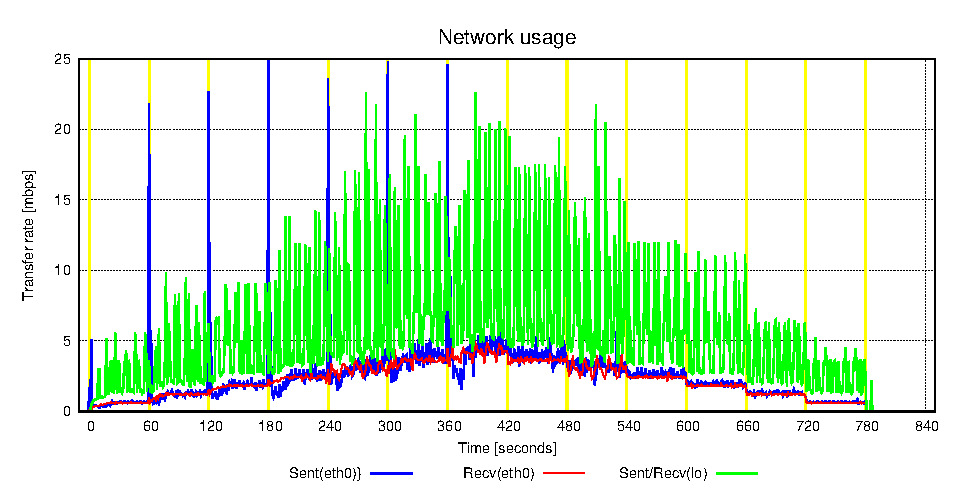
\includegraphics[width=\linewidth]{stats/test_full_features_net.eps}
  \caption{Network usage after implementing all features}
  \label{fig:test_full_features_net}
\end{figure}


      The blue peaks are caused by the signaling phase and web page downloads, including resources such as images, stylesheets and javascript files. 
      The green peaks are caused by video and audio being transfered between \gls{KMS} and \emph{MongoDB} through \emph{Kurento Repository}. Each peak occurs every time a block of video is recorded, which in this case is every ten seconds. 
      The recordings are synchronized so all user and mixed blocks start and end at the same time. That is why the amount of work done every ten seconds accumulates, and because this is performed locally, the maximum transfer rate is limited by the performance of the memory as buffers are written to buffers then to disks. 
      Sent data transfer rate has no significant peaks as \gls{HTTP} requests and signaling information contains little information.

	With this results we conclude that if we want to scale our storage solution using the \emph{MongoDB}'s cluster configuration, both \emph{Kurento Repository} and \gls{KMS} should be installed on the same machine because the loopback interface can handle bigger transfer rates than the remaining network interfaces. Installing the repository on the same machine as a database node does not ensure that recorded videos are stored in the same machine, for this reason we would prefer installing \gls{KMS} and \emph{Kurento Repository} on the same machine.





On the other hand, Figure \ref{fig:test_client_net} shows the respective network usage on the client side during our test case. We observe that in the first seconds the client adjusts the video quality it sends to \gls{KMS}. Whenever a new client enters the conference, we observe that \gls{KMS} decreases the video quality in order to instantaneously integrate a new user into the conference room. After a while, \gls{KMS} realizes that the network can handle the increase of clients and sends the video with a better quality to every participant. When a user leaves the conference room \gls{KMS} has no need to decrease the participant's video quality as less network bandwidth will be used.

\begin{figure}
  \centering
  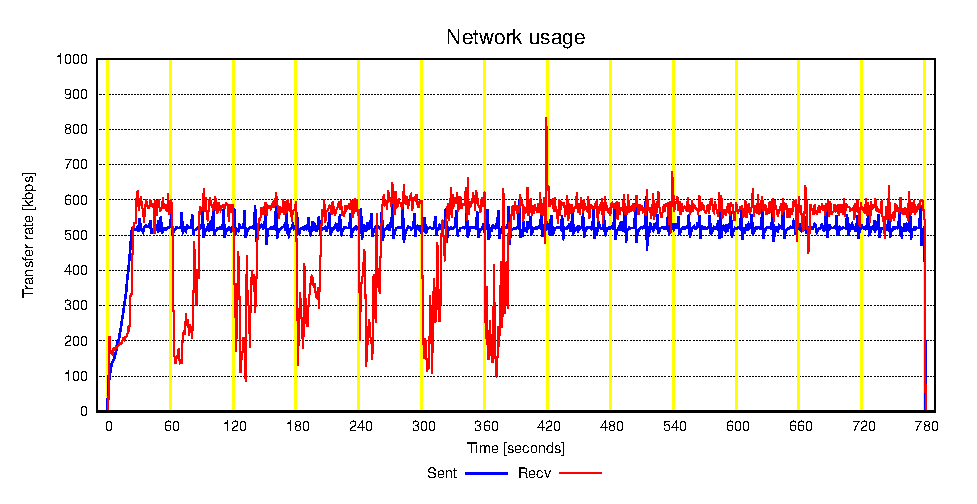
\includegraphics[width=\linewidth]{stats/test_client_net.eps}
  \caption{Client Network usage during our test case}
  \label{fig:test_client_net}
\end{figure}



\textbf{Memory usage}


Figure \ref{fig:test_ram_fixed_mem} shows the memory usage during our performance test. Both \gls{JVM}, \emph{MongoDB} and \gls{KMS} performs their own memory management by holding and recycling objects when needed. The expected and observed behavior of the memory usage is growth of memory usage while the users are entering the conference room and a memory usage stabilization afterwards.


\begin{figure}
  \centering
  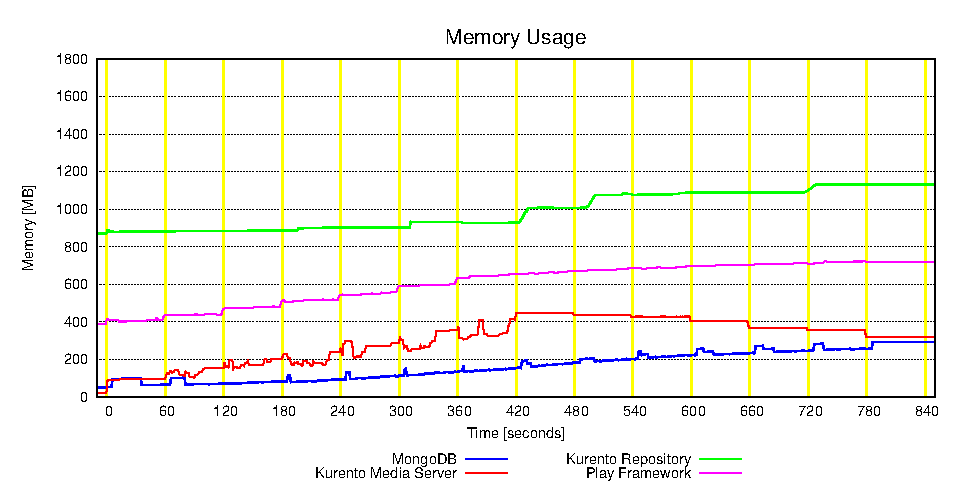
\includegraphics[width=\linewidth]{stats/test_ram_fixed_mem.eps}
  \caption{Memory usage after fixing recorder memory leak}
  \label{fig:test_ram_fixed_mem}
\end{figure}

\emph{MongoDB} memory usage keeps increasing because it tries to fit part of the database on \gls{RAM} for fast read access. \emph{MongoDB} checkpoints data to disk every 60 seconds or when journal data exceeds 2GB\footnote{\url{https://docs.mongodb.org/manual/faq/storage/}(Accessed March 28, 2016)}, that explains the small memory usage peaks during our test case. When the conference room is empty there are no video recordings, which explains the memory stabilization at the end.

\emph{KMS} memory management released resources as soon as users left the room. 


\textbf{CPU usage}


Figure \ref{fig:test_full_features_cpu} shows the percentage of \gls{CPU} usage during our performance test case. Each 100\% represents one \gls{CPU} core, although that does not mean one \gls{CPU} is fully used, for example two cores at 60\% represent 120\% \gls{CPU} usage. As we can see, the percentage of \gls{CPU} used increases and decreases linearly in function of the amount of conference participants. \gls{KMS} is responsible for most \gls{CPU} usage.


\begin{figure}
  \centering
  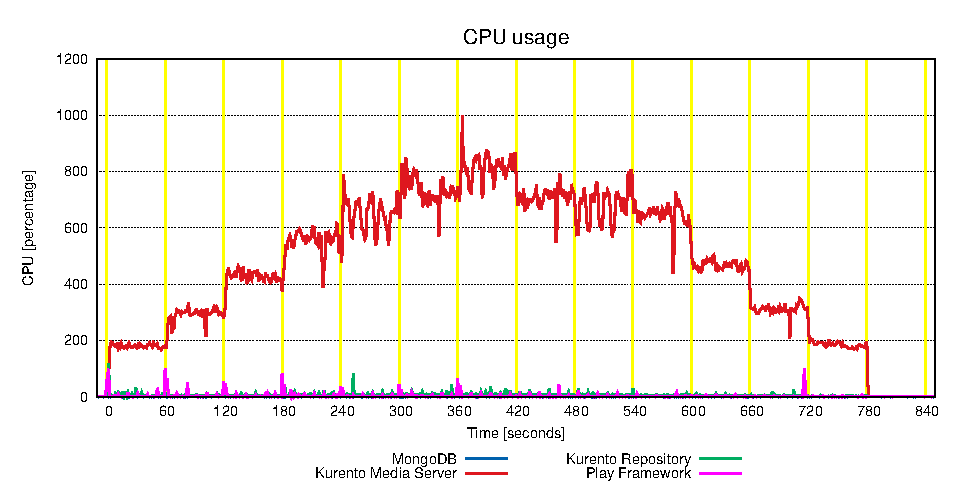
\includegraphics[width=\linewidth]{stats/test_full_features_cpu.eps}
  \caption{Percentage of CPU used during the performance tests}
  \label{fig:test_full_features_cpu}
\end{figure}

  Just for testing purposes, we performed the same performance tests disabling \gls{QR} codes detection. We concluded that \gls{QR} code detection is a very intensive task, approximately doubling the amount of work performed by the \gls{CPU}s.

	Even though, with this test results, we conclude that our solution's bottleneck is the \gls{CPU} usage at \gls{KMS}.



\subsection {Usability Tests}
     In this section we describe usability test scenarios that we have applied and their respective results.


    \subsubsection{Tests Scenarios}

      In order to evaluate the usability of our solution, we have performed usability tests with the help of real users with different backgrounds and ages.

      We handed a guide to the users with five tasks to perform. The metrics we used for each task were: number of clicks, number of errors (including a description) and time spent. 

  \subsubsection{Test Results}

In this section we present the results of our usability tests. The first time we tested our solution by providing tasks to users, we have observed that our solution was not perfect. Having faced usability problems during our tests, he had to improve our solution's usability and start the tests again.


In the first testing phase we have performed tests with just three users and ceased for improvements. We gathered comments and suggestions after letting the users explore our system.

On the second phase of our user interface tests, in a general way, we have noticed great improvements on the learning time.

In order to measure the users learning speed, we have performed tests with experienced users in order to retrieve the optimal task duration and minimal task clicks.

To this end, with regard to optimal task duration and minimal clicks, we obtained the values shown in Table \ref{table:optimal}.


\begin{table}[H]
\centering
\caption{Metrics for an experienced user}
\label{table:optimal}
\begin{tabular}{|c|c|c|c|c|c|}
\hline
\textbf{Task} & 1 & 2 & 3 & 4 & 5 \\ \hline
\textbf{Duration (seconds)} & 20 & 35 & 30 & 25 & 35 \\ \hline
\end{tabular}
\end{table}


From the data collected with twenty tests with users, namely the task duration (Figure \ref{fig:user_times}) and task difficulty (Figure \ref{fig:user_diffs}), we have calculated the confidence intervals in order to understand the most plausible values for each metric.

The youngest and oldest testers were, receptively, twenty two and thirty eight years old. Figure \ref{fig:user_ages} the ages of the users that tested our system.

\begin{figure}
  \centering
  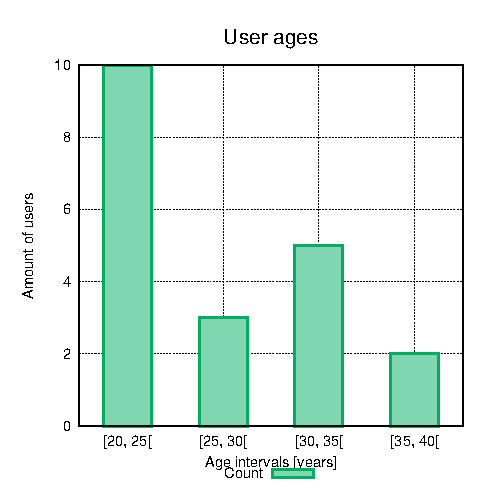
\includegraphics[width=0.8\linewidth]{stats/user_ages.eps}
  \caption{Ages of the users that tested our system}
  \label{fig:user_ages}
\end{figure}

As a result of both true average and variance being unknown and the usage of a relatively small amount of samples, we had to use \emph{t-distribution} to estimate our metrics confidence intervals. We have used a 95\% confidence level.

\begin{figure}
  \centering
    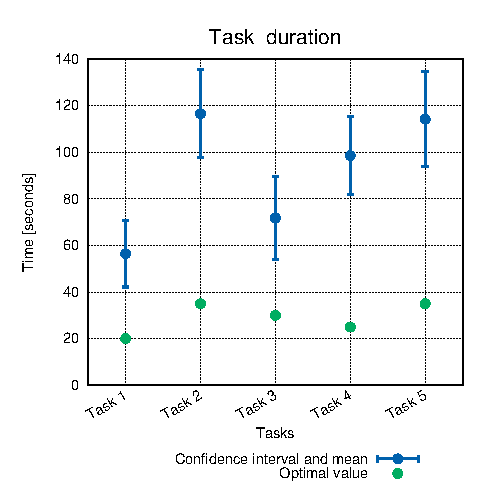
\includegraphics[width=0.8\linewidth]{stats/user_times.eps}
    \caption{Time spent per task}
    \label{fig:user_times}
\end{figure}

According to Figure \ref{fig:user_diffs}, we can observe that most users had less difficulties with the first two tasks, which represents types of tasks that most users are familiar with. As soon as users had to navigate in time, manipulate annotations and create content (respectively \emph{task3}, \emph{task4} and \emph{task5}) we observed that they revealed more difficulties. Most of those difficulties, based on the users feedback, were mainly due to those concepts not being familiar to them.



\begin{figure}
  \centering
    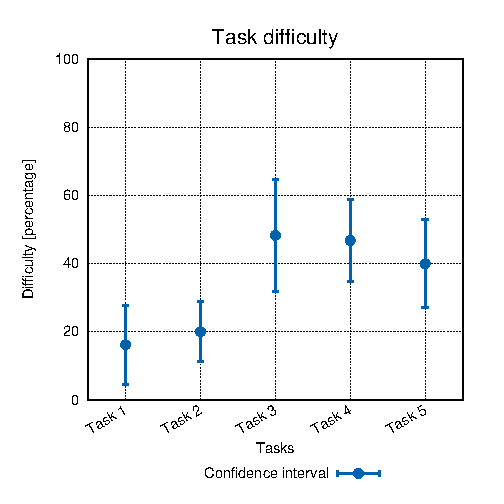
\includegraphics[width=0.8\linewidth]{stats/user_diffs.eps}
  \caption{Difficulty per task}
  \label{fig:user_diffs}
\end{figure}


As we had relatively bad results with some users, we explained to those users that could not conclude the tasks or performed them incorrectly, the most efficient way to perform the requested tasks. Some users suggested to display more hints in order to achieve a faster learning, but afterwards all were impressed and gave us a better evaluation.

Most users gave us worse evaluations on our user interface layout and content editor, which was due to having a lot of tools present in the same web page and some of them being hidden due the screen size. In some cases users had to scroll down in order to find the tools they were looking for. 

Another weak aspect was our content editor, which, in fact, we recognize is difficult to work with, mostly due to the amount of information that is necessary to create a synchronized content (starting time, duration and content itself). Some users have suggested that the content should also be present on the timeline so they could be easily dragged and resized (on time).

We are aware that placing content on the timeline will reduce our solutions performance, especially when there is a relatively large amount of content, due to the content that is present on the timeline being loaded all at once. Although, we recognize that for some cases (relatively low amount of content), displaying the content on the timeline could not have a great impact on our solutions performance, we choose not to implement this.

In conclusion, 100\% of our testers though that our solution was an innovation and 95\% recommended using our solution.
















\section{Conclusions}
\label{chapter:conclusion}
\subsection{Achievements}
\label{section:achievements}

	We have successfully implemented the basic functionalities of our prototype and spare some time for adding more valuable features such as the ability to create content by exposing \gls{QR} codes to the camera and lastly perform changes to the user interface in order to improve the quality of user's experience.

	The performance tests that we have executed showed that our system is stable and more importantly that our web server is lightweight and most of processing power is dedicated to the streaming server.

	Our usability tests show results that are considerably worse than the established optimal values due to our solution propose a different way to communicate that most people are not used to. Although we have obtained those results, in general our users gave us positive feedback and valuable advices which we have used to improve our system. 

\subsection{Future Work}
\label{section:future}
	Playing back video with a faster rate is not possible using the current version of \gls{KMS}. Even though we expect the availability of that feature in a near future but we have proposed an alternative way to implement faster playback by using \emph{ffmpeg} to convert the video before playing it.

	Although we have tested our solution in a powerful machine for the current time, our performance tests revealed that the streaming component uses a lot of resources. We left for a future work a deep analysis on the scalability of our system for which we have proposed different approaches but we have not tested them.

	Another aspect we could have tested was the performance of our solution when using \gls{TURN} servers for relaying the traffic that fails using \gls{STUN}.

	Lastly, we have chosen functionality over security in respect to displaying content to users which lead to security flaws on our solution. Although we have not solved the security problems, we have proposed a solution which at the same time limits the flexibility of adding new functionalities to our prototype.


% trigger a \newpage just before the given reference
% number - used to balance the columns on the last page
% adjust value as needed - may need to be readjusted if
% the document is modified later
%\IEEEtriggeratref{8}
% The "triggered" command can be changed if desired:
%\IEEEtriggercmd{\enlargethispage{-5in}}


\bibliographystyle{IEEEtran}
\bibliography{../tese2/references}


\end{document}


